% Created 2025-02-04 mar. 12:08
% Intended LaTeX compiler: pdflatex
\documentclass[11pt]{article}
\usepackage[utf8]{inputenc}
\usepackage[T1]{fontenc}
\usepackage{graphicx}
\usepackage{longtable}
\usepackage{wrapfig}
\usepackage{rotating}
\usepackage[normalem]{ulem}
\usepackage{amsmath}
\usepackage{amssymb}
\usepackage{capt-of}
\usepackage{hyperref}
\usepackage{listings}
\usepackage{lmodern} % Ensures we have the right font
\usepackage{graphicx}
\usepackage{amsmath, amsthm, amssymb}
\usepackage[table, xcdraw]{xcolor}
\usepackage{fancyhdr}
\usepackage[lined,boxed,commentsnumbered,ruled,vlined,linesnumbered]{algorithm2e}
\SetKwComment{Comment}{$\triangleright$\ }{}
\usepackage[left=2cm,right=2cm,top=3cm,bottom=3cm]{geometry}
\pagestyle{fancy}
\makeatletter
\edef\mytitle{\@title}
\makeatother
\fancyhead{} % clear all fields
\fancyhead[L]{\slshape \rightmark}
\renewcommand{\headrulewidth}{0.1pt}
\fancyfoot{} % clear all fields
\fancyfoot[R]{Page \thepage}
\renewcommand{\footrulewidth}{0pt}
\usepackage{titling}
\setlength{\droptitle}{-8ex}
\pretitle{\begin{flushleft}\Large\bfseries}
\posttitle{\par\end{flushleft}}
\preauthor{\begin{flushleft}\large}
\postauthor{\end{flushleft}}
\predate{\begin{flushleft}}
\postdate{\end{flushleft}}
\usepackage[normalem]{ulem}
\usepackage{sectsty}
\sectionfont{\underline}
\makeatletter
\def\@seccntformat#1{%
\expandafter\ifx\csname c@#1\endcsname\c@section\else
\csname the#1\endcsname\quad
\fi}
\makeatother
\usepackage[font={color=gray},figurename=Fig.,labelfont={it}]{caption}
\usepackage{enumitem}
\setlist{noitemsep}
\setlist{itemsep=-10pt}
\usepackage{listings}
\usepackage{tikz}
\usepackage{lstautogobble}  % Fix relative indenting
\usepackage{color}          % Code coloring
\usepackage{zi4}            % Nice font

\definecolor{bluekeywords}{rgb}{0.13, 0.13, 1}
\definecolor{greencomments}{rgb}{0, 0.5, 0}
\definecolor{redstrings}{rgb}{0.9, 0, 0}
\definecolor{graynumbers}{rgb}{0.5, 0.5, 0.5}
\definecolor{grayW}{rgb}{0.96,0.96,0.97}

\usepackage{listings}
\lstset{
backgroundcolor=\color{grayW},
autogobble,
columns=fullflexible,
showspaces=false,
showtabs=false,
breaklines=true,
showstringspaces=false,
breakatwhitespace=true,
escapeinside={(*@}{@*)},
commentstyle=\color{greencomments},
keywordstyle=\color{bluekeywords},
stringstyle=\color{redstrings},
numberstyle=\color{graynumbers},
basicstyle=\ttfamily\footnotesize,
frame=tlbr,
framesep=12pt,
xleftmargin=12pt,
tabsize=4,
captionpos=b,
framexleftmargin=15pt,
framerule=0pt
}
\setlength{\arrayrulewidth}{0.3mm}
\setlength{\tabcolsep}{3pt}
\renewcommand{\arraystretch}{1.2}
\usepackage[skip=0pt, parfill]{parskip}
\usepackage{tocloft}
\renewcommand{\cftsecleader}{\cftdotfill{\cftdotsep}}
\usepackage{indentfirst}
\usepackage[fontsize=10pt]{fontsize}
\usepackage{setspace}
\setstretch{1,25}
\usepackage{forest}
\usepackage[linesnumbered]{algorithm2e}
\author{Author: Enzo Durel \newline }
\date{\today}
\title{5043 Advanced Machine Learning - HW 0}
\hypersetup{
 pdfauthor={Author: Enzo Durel \newline },
 pdftitle={5043 Advanced Machine Learning - HW 0},
 pdfkeywords={},
 pdfsubject={},
 pdfcreator={Emacs 29.4 (Org mode 9.6.15)}, 
 pdflang={English}}
\begin{document}

\maketitle


\begin{center}
\includegraphics[width=10cm]{/home/hozen/orgmode_latex_export_img/ou_logo.png}
\end{center}\\[0pt]

\thispagestyle{empty}
\setcounter{tocdepth}{3}
\tableofcontents
\clearpage
\pagenumbering{arabic}

\thispagestyle{empty}
\listoffigures
\clearpage
\pagenumbering{arabic} 

\newpage

\section{Report}
\label{sec:orgf58578d}
\subsection{Design}
\label{sec:org1aaadd1}

\noindent \uline{Activation function}: I choose to use the tanh activation because the range of the outputs is [-1,1].\\[0pt]
\uline{Number of hidden layers}: I choose to get more hidden layer but not increase their size.\\[0pt]
\uline{Learning rate}: I opt for a lrate = 0.0005.\\[0pt]
\uline{Epochs}: Because of my learning rate is low, I opt for more epochs with a possibility of a callback that stop training if the efficiency of the neural network does not increase.\\[0pt]

\subsection{Plots}
\label{sec:orgeecdf26}
\subsubsection{Learning Curves}
\label{sec:org3e5c61b}

Here is the curves of learning of the models.\\[0pt]

\begin{figure}[htbp]
\centering
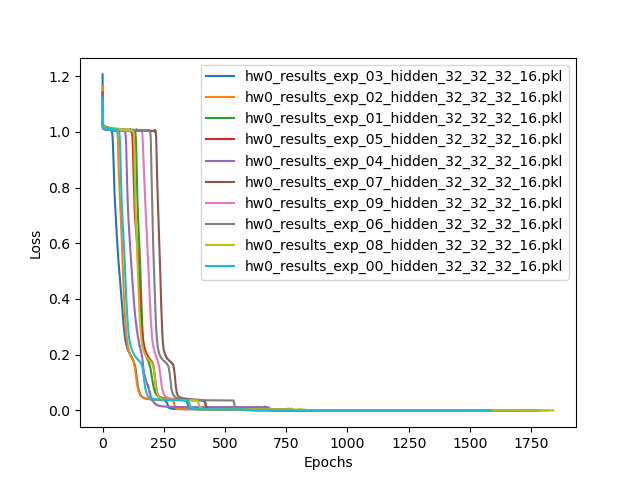
\includegraphics[width=10cm]{img/learning_curves.png}
\caption{Learning Curves of 10 models}
\end{figure}\\[0pt]

\subsubsection{Error Histogram}
\label{sec:org01a1550}

Here is the historgram representing the number of absolute error counted in the model prediction. The goal here is to have only absolute error less than 0.1.\\[0pt]

\begin{figure}[htbp]
\centering
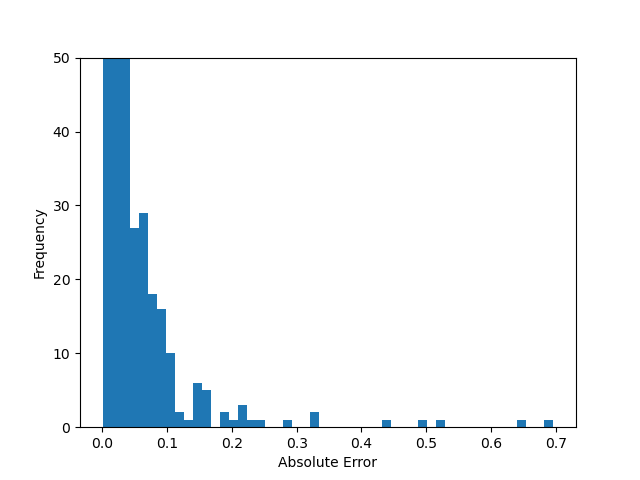
\includegraphics[width=10cm]{img/error_histogram.png}
\caption{Error Histogram of 10 models}
\end{figure}\\[0pt]

\subsubsection{Absolute Errors}
\label{sec:org87025f4}

Here are the different bars for each run, corresponding respectively for a model as: the sum of the absolute errors, the maximum of the absolute errors, and the count of absolute errors greater than 0.1.\\[0pt]

\begin{figure}[htbp]
\centering
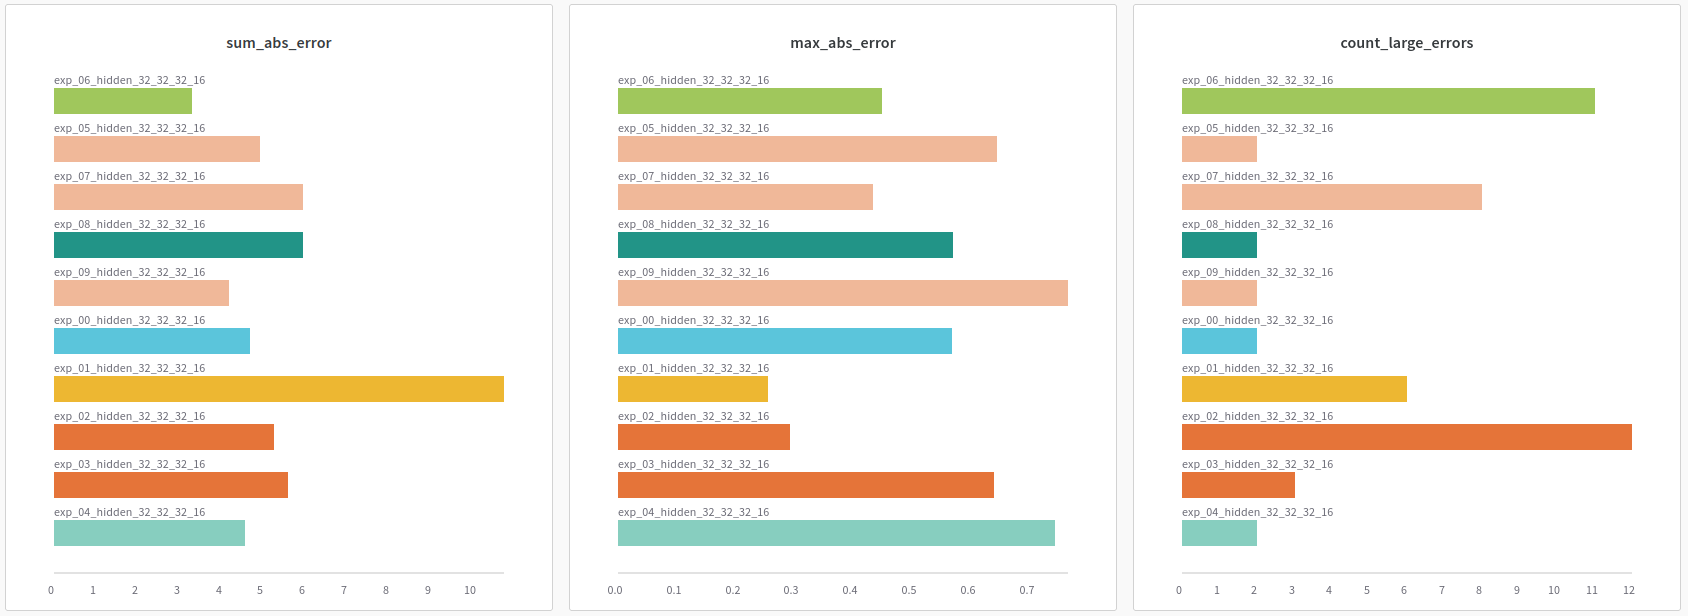
\includegraphics[width=.9\linewidth]{img/bar_errors.png}
\caption{Absolute Errors per run}
\end{figure}\\[0pt]
\end{document}
